\documentclass[a4paper,12pt]{article}
\usepackage{amsmath}
\usepackage{amssymb}
\usepackage[utf8]{inputenc}
\usepackage[T1]{fontenc}
\usepackage{lmodern}
\usepackage{indentfirst}
\usepackage{geometry}
\usepackage{array}
\usepackage[pdftex]{color,graphicx}
\usepackage{subfigure}
\usepackage{afterpage}
\usepackage{setspace}
\usepackage{color}
\usepackage{wrapfig}
\usepackage{listings} 
\usepackage{datetime}
\usepackage{epstopdf}
\usepackage{hyperref}

\renewcommand{\onehalfspacing}{\setstretch{1.6}}

\geometry{tmargin=2.5cm,bmargin=2.5cm,lmargin=2.5cm,rmargin=2.5cm}
\setlength{\parindent}{1cm}
\setlength{\parskip}{0mm}

\newenvironment{lista}{
\begin{itemize}
  \setlength{\itemsep}{1pt}
  \setlength{\parskip}{0pt}
  \setlength{\parsep}{0pt}
}{\end{itemize}}

\newcommand{\linia}{\rule{\linewidth}{0.4mm}}

\definecolor{lbcolor}{rgb}{0.95,0.95,0.95}
\lstset{
  backgroundcolor=\color{lbcolor},
  tabsize=4,
  language=C++,
  captionpos=b,
  tabsize=3,
  frame=lines,
  numbers=left,
  numberstyle=\tiny,
  numbersep=5pt,
  breaklines=true,
  showstringspaces=false,
  basicstyle=\footnotesize,
  identifierstyle=\color{magenta},
  keywordstyle=\color[rgb]{0,0,1},
  commentstyle=\color{green},
  stringstyle=\color{red}
  }

\begin{document}

\noindent
\begin{tabular}{|c|p{11cm}|c|} \hline 
Michał Szczygieł & Aleksander Śmierciak & \ddmmyyyydate\today \tabularnewline
\hline 
\end{tabular}


\section*{Zadanie 1 - Macierze OMP}

\textit{Proszę sprawdzić jak różni się czas mnożenia i dodawania macierzy. Który problem, dodawanie czy mnożenie wart jest zrównoleglenia?}
\\


Mnożenie jest operacją arytmetyczną bardziej kosztowną od dodawania, więc to właśnie ta operacja jest bardziej warta zrównoleglania. Ponadto, mnożenie macierzy samo w sobie jest bardziej skomplikowane algorytmicznie niż ich dodawanie.
\\


\textit{Jaki wpływ na zrównoleglenie będzie miało zastosowanie poniższej dyrektywy OpenMP:}
\begin{lstlisting}
#pragma omp parallel for default(shared)
\end{lstlisting}

\textit{a jaki dyrektywa:}

\begin{lstlisting}
#pragma omp parallel for default(none) shared(A, B, C) firstprivate(rozmiar) private(i, j)
\end{lstlisting}

Klauzula default określa tryb współdzielenia zmiennych w obszarze równoległym OpenMP. Wartość ‘shared’, która jest wartością domyślną, oznacza że każda zmienna znajdująca się w obszarze równoległym będzie traktowana jak gdyby była oznaczona klauzulą shared.
Wartość ‘none’ oznacza, że każda zmienna zadeklarowana poza obszarem równoległym, nieokreślona jedną z klauzul: private, shared, reduction, firstprivate, lastprivate i użyta w tym obszarze spowoduje błedy kompilacji.
\\

Pierwsza postać dyrektywy określa wszystkie zmienne obszaru równoległego jako współdzielone między wątkami.
Druga postać dyrektywy określa zmienne A, B i C jako współdzielone, zmienną rozmiar jako prywatną o wartości wprowadzanej do obszaru równoległego i zmienne i, j jako zmienne prywatne bez wartości początkowej, a każde inne w obszarze równoległym wykorzystywane spowodują błędy kompilacji.
\\

Poniżej został umieszczony wycinek kodu odpowiedzialny za mnożenie macierzy.

\begin{lstlisting}
const DoubleMatrix *multiplyMatrices(const DoubleMatrix &A, const DoubleMatrix &B, unsigned int threadCount)
{
    assertSizeEqual(A, B);

    DoubleMatrix *C = new DoubleMatrix();
    fillMatrixWithZeros(*C, A.size());
    unsigned int rowSize = sqrt(A.size());

    #pragma omp parallel for default(none) shared(A, B, C) firstprivate(rowSize) num_threads(threadCount)
    for (unsigned int i = 0; i < rowSize; ++i)
    {
        //double local = 0.0;
        for (unsigned int j = 0 ; j < rowSize; ++j)
        {
            C->at(i * rowSize + j) = A.at(i * rowSize + j) * B.at(i + j * rowSize);
            //local += A.at(i * rowSize + j) * B.at(i + j * rowSize);
        }
    }

    return C;
}
\end{lstlisting}

Poniżej został umieszczony wycinek kodu odpowiedzialny za sumowania macierzy.
\begin{lstlisting}
const DoubleMatrix *sumMatrices(const DoubleMatrix &A, const DoubleMatrix &B, unsigned int threadCount)
{
    assertSizeEqual(A, B);

    DoubleMatrix *C = new DoubleMatrix();
    fillMatrixWithZeros(*C, A.size());

    #pragma omp parallel for default(none) shared(A, B, C) num_threads(threadCount)
    for (unsigned int i = 0; i < A.size(); i++)
    {
        C->at(i) = A.at(i) + B.at(i);
    }

    return C;
}
\end{lstlisting}

Poniżej wykresy przedstawiający rezultat przeprowadzonych operacji na wątkach.
\\
\begin{center}
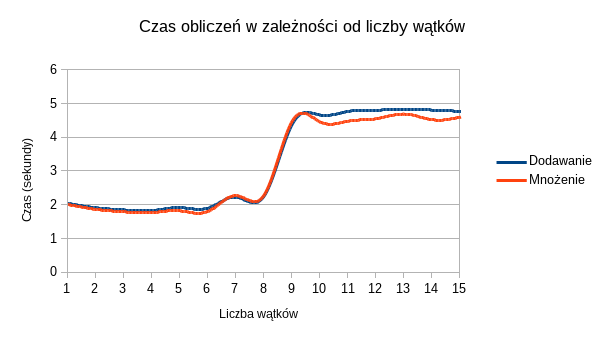
\includegraphics[width=0.7\textwidth]{data/czas.png}
\end{center}

\begin{center}
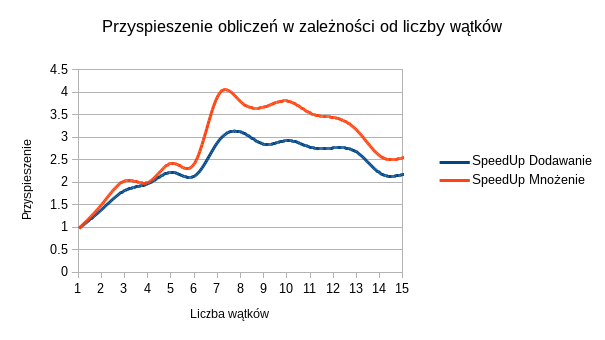
\includegraphics[width=0.7\textwidth]{data/przysp.png}
\end{center}

\section*{Wnioski}
Przy użyciu OpenMP możemy zrównoleglić każdy powtarzalny fragment kodu uzyskując przy tym wysoką wydajność na maszynach wielordzeniowych. 
Wraz ze wzrostem liczby wątków obserwujemy spadek czasu potrzebnego na wykonanie programu. Ten wzrost nie jest jednak liniowy - dla pewnej liczby wątków funkcja przyspieszenia stabilizuje się. Jest to związane z osiągnięciem stanu, w którym tworzenie kolejnych wątków, ich synchronizacja i zarządzanie są operacjami o kosztach przewyższających zyski ze zrównoleglania wykonywanych obliczeń.
Innym wytłumaczeniem - być może kolejnym - jest nieregularne obciążenie serwera, na którym pomiary były wykonywane

\end{document}
